\chapter{Humanoids and steerable WMRs}
\label{ch:humanoids-and-swmrs}
Todo. 

\begin{figure}
    \centering
    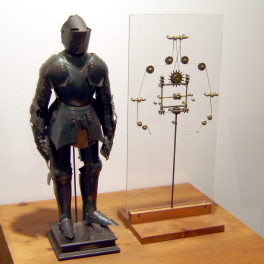
\includegraphics[width=\textwidth]{figures/01-introduction/robot-history.jpg}
    \caption{From left to right: Leonardo's robot, constructed by Leonardo Da
        Vinci in 1495 \cite{Moran2006TheDaVinciRobot};
        R.U.R. (Rossum's Universal Robots) by Karel {\v C}apek introduced 
        the word ``robot'' in 1920 \cite{Capek1920RUR};
        C-3PO, the famous humanoid robot from the Star Wars Cinematic Universe
        \cite{StarWars1977}.
    }
    \label{fig:introduction:robots-in-history}
\end{figure}

\begin{figure}
    \centering
    
\includegraphics[width=\textwidth]{figures/01-introduction/robots-in-animation.jpg}
    \caption{Humanoid robots in animation. From left to right:
        The Iron Giant (1999) \cite{TheIronGiant1999},
        Bender from Futurama (1999) \cite{Futurama1999}, and
        Baymax from Big Hero 6 (2014) \cite{BigHero62014}.
    }
    \label{fig:introduction:robots-in-animation}
\end{figure}

\begin{figure}
    \centering
    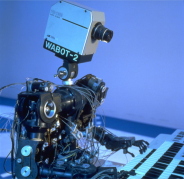
\includegraphics[width=0.7\textwidth]{figures/01-introduction/WABOTs.jpg}
    \caption{From left to right: the WABOT-1 (1972), which is the first anthropomorphic robot
        ever developed \cite{Kato1973TheWABOT1}, and the WABOT-2 (1984)
        playing a keyboard \cite{Kato1987WABOT2}.}
    \label{fig:introduction:WABOTs}
\end{figure}

\begin{figure}
    \centering
    \includegraphics[width=0.7\textwidth]{figures/01-introduction/The-ASIMO-humanoid-robot-history.png}
    \caption{Honda E series (E0 in 1986 to E6 in 1993) robots, Honda P series (P1 in
        1993 to P3 in 1997) robots, and ASIMO (2000)
        \cite{Shigemi2019ASIMOandHumanoidRobotResearchatHonda}.}
    \label{fig:introduction:ASIMO-humanoid-history}
\end{figure}

\begin{figure}
    \centering
    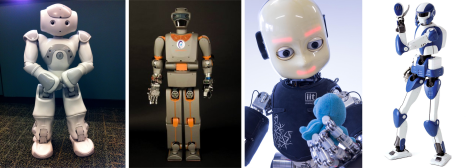
\includegraphics[width=\textwidth]{figures/01-introduction/robots-in-2000.jpg}
    \caption{Some of the humanoid robots developed in 2000s. From left to right:
        Aldebaran NAO \cite{Gouaillier2008NAOHumanoid},
        PAL Robotics REEM-B \cite{Tellez2008REEMB},
        iCub \cite{Metta2010iCubHumanoid}, and
        HRP-4 \cite{Kaneko2011HRP4}.
    }
    \label{fig:introduction:robots-in-2000}
\end{figure}

\begin{figure}
    \centering
    \includegraphics[width=\textwidth]{figures/01-introduction/robots-in-2010.jpg}
    \caption{Some of the humanoid robots developed in 2010s. From left to right:
        Boston Dynamics ATLAS,
        WALK-MAN \cite{Tsagarakis2017WALKMAN},
        NASA Valkyrie \cite{Radford2015Valkyrie}, and
        PAL Robotics TALOS \cite{Stasse2017TALOS}.}
    \label{fig:introduction:robots-in-2010}
\end{figure}

\begin{figure}
    \centering
    \includegraphics[width=\textwidth]{figures/01-introduction/robots-in-2020.jpg}
    \caption{Some of the humanoid robots developed in 2020s for commercial
        purposes. From left to right:
        Digit by Agility Robotics, Optimus by Tesla, Apollo by Apptronik, and
        Figure 01 by Figure AI.
    }
    \label{fig:introduction:robots-in-2020}
\end{figure}

\begin{figure}
    \centering
    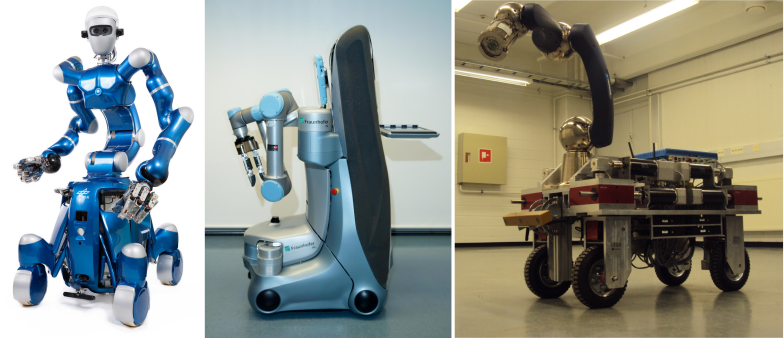
\includegraphics[width=\textwidth]{figures/01-introduction/SWMRs-1.jpg}
    \caption{Robots equipped with steerable wheels to be deployed in different areas.
        From left to right: Rollin' Justin \cite{Fuchs2009RollinJustin}, used 
        for household work and astronauts assistance in space, 
        Care-O-bot 3 \cite{Graf2009Care-O-bot3}, used as service robot, and
        iMoro \cite{Oftadeh2013iMoro}, used for inspection of contaminated
        environments.}
    \label{fig:introduction:SWMRs-1}
\end{figure}

\begin{figure}
    \centering
    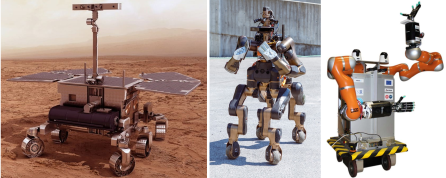
\includegraphics[width=\textwidth]{figures/01-introduction/SWMRs-2.jpg}
    \caption{More recent robots equipped with steerable wheels.
        ExoMars \cite{Poulakis2015ExoMarsMobilitySubsystem}, conceived for 
        space exploration,
        CENTAURO \cite{Kashiri2019Centauro}, designed for loco-manipulation
        in disaster scenarios, and
        BAZAR \cite{Cherubini2019ACR}, designed to interact with humans in
        assembly lines.
    }
    \label{fig:introduction:SWMRs-2}
\end{figure}
